\documentclass[11pt]{article}
\usepackage{graphicx, subfig}
\usepackage[top=1in, bottom=1in, left=1in, right=1in]{geometry}
\graphicspath{ {./figs/} }
\pagestyle{plain}
\begin{document}
\title{\vspace{-5mm}Voting Model and Edge Reconnecting Model CPI}
\author{Alexander Holiday}
\maketitle
\section*{Voting model}
\begin{figure}
  \centering
  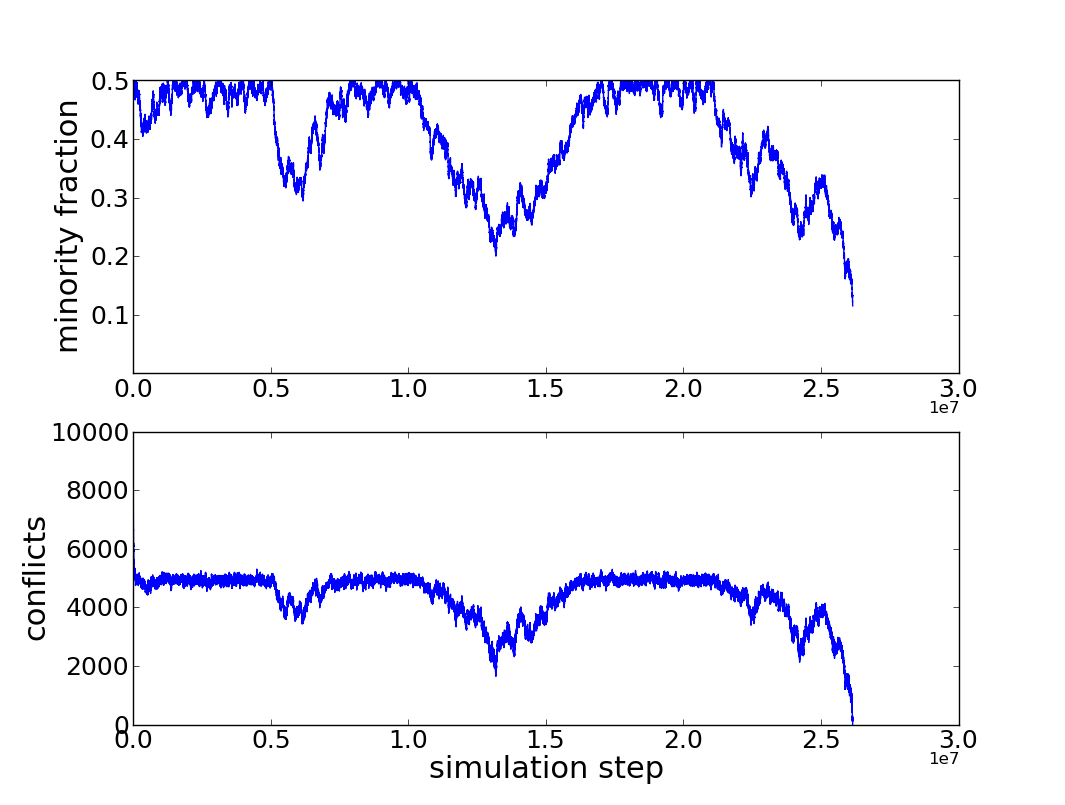
\includegraphics[height=65mm]{vmDynamics}
  \caption{Evolution of conflicts and minority fraction in a single voting model simulation.}
  \label{fig:vmDynamics}
\end{figure}

\begin{figure}
  \centering
  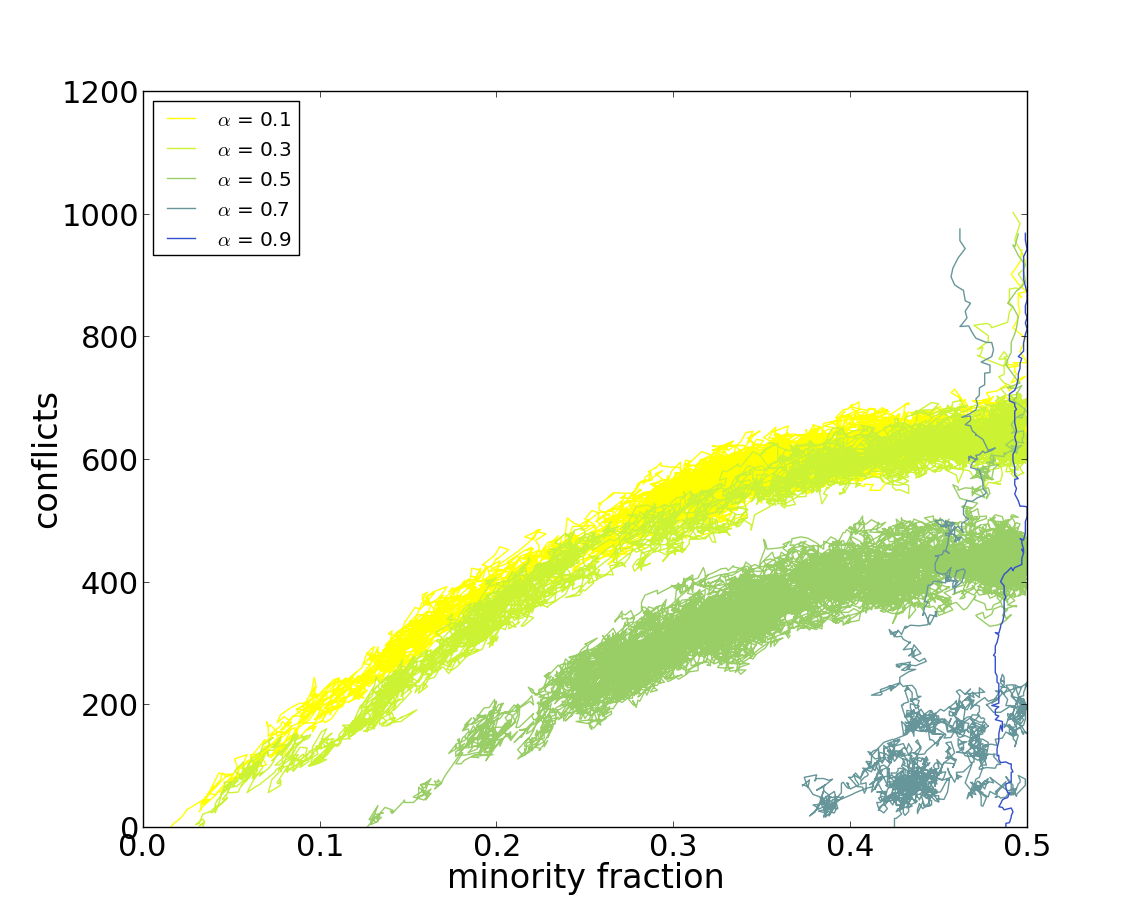
\includegraphics[height=65mm]{vmPhasePortrait}
  \caption{Phase portrait at varying values of $\alpha$.}
  \label{fig:vmPP}
\end{figure}

\begin{figure}
  \centering
  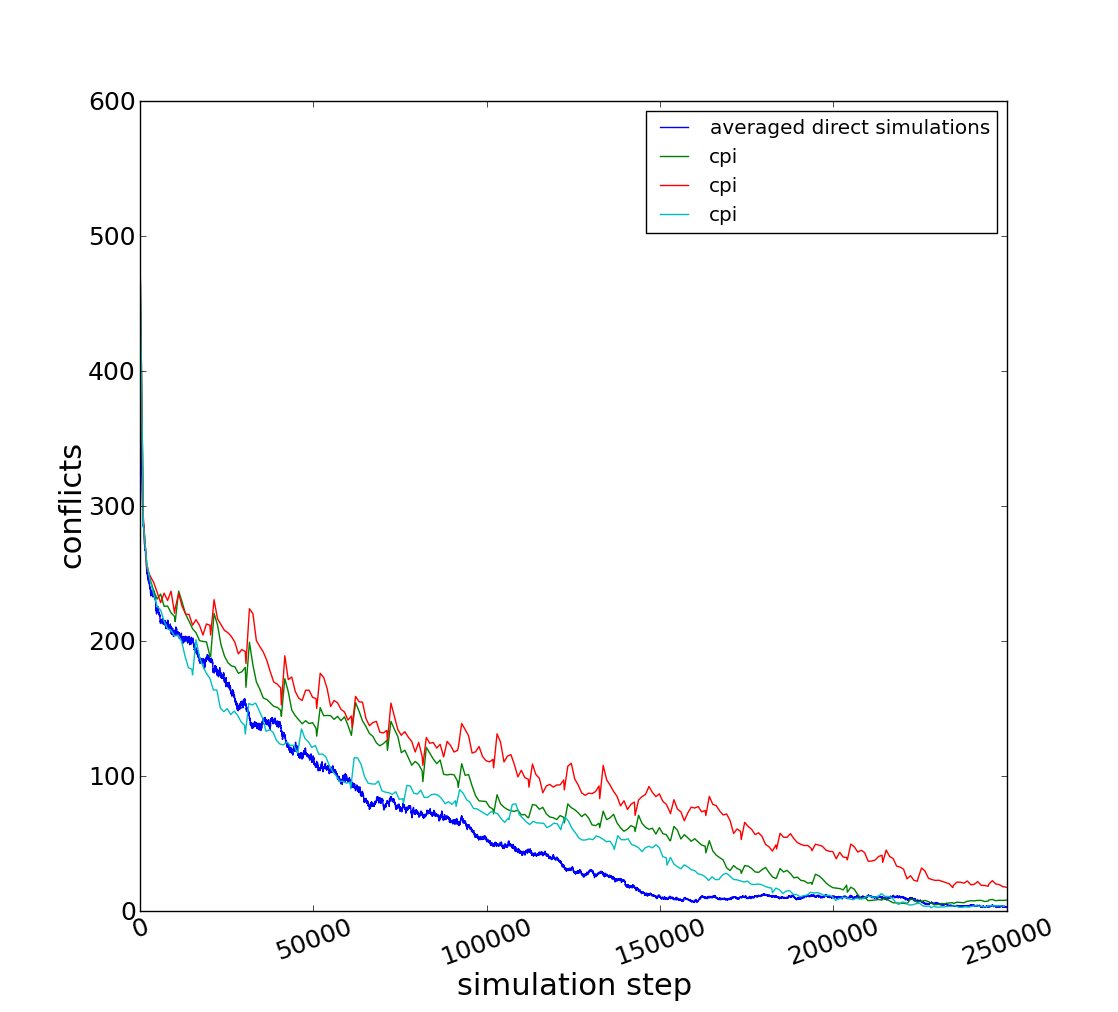
\includegraphics[height=65mm]{vmHealing}
  \caption{``Healing'' of voting model back to slow manifold, simulation was restricted and immediately lifted every $10,000$ steps.}
  \label{fig:vmHealing}
\end{figure}

\begin{figure}
  \centering
  \subfloat[Evolved $1000$ steps, projected $200$.]{
    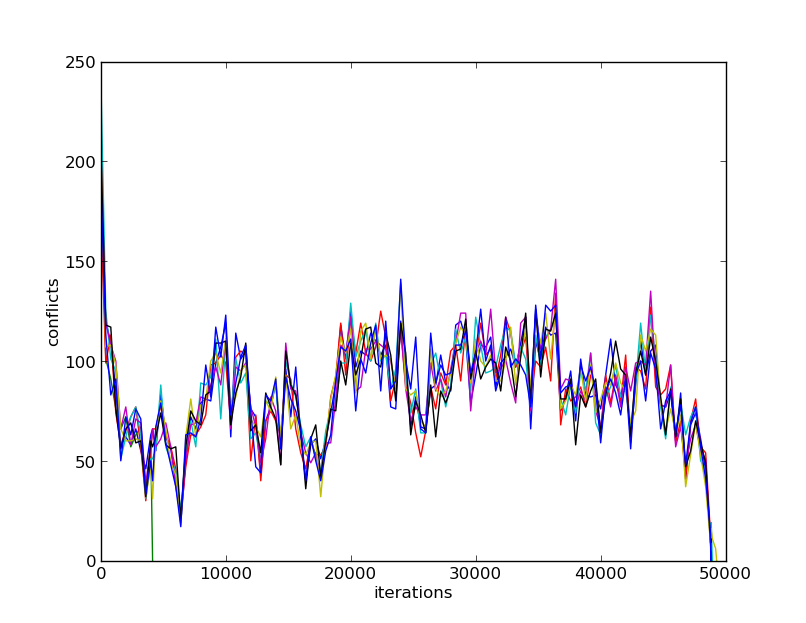
\includegraphics[height=65mm]{vmCPISlow1}
    \label{fig:vmSlow1}
  }
  \hspace{3mm}
  \subfloat[Evolved $1000$ steps, projected $200$.]{
    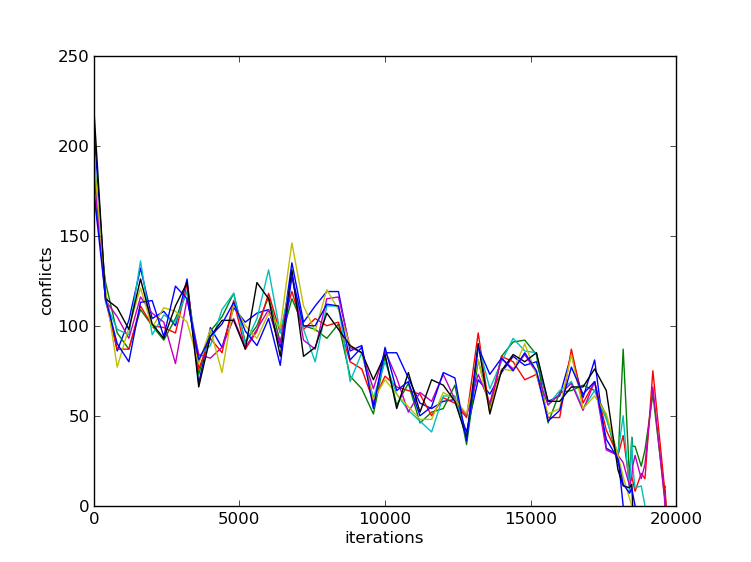
\includegraphics[height=65mm]{vmCPISlow2}
    \label{fig:vmSlow2}
  }
  \caption{First CPI method in which finished runs in the ensemble are entirely removed from the simulation. This causes slower convergence.}
  \label{fig:vmSlow}
\end{figure}

\begin{figure}
  \centering
  \subfloat[Evolved $15,000$ steps, projected $5,000$.]{
    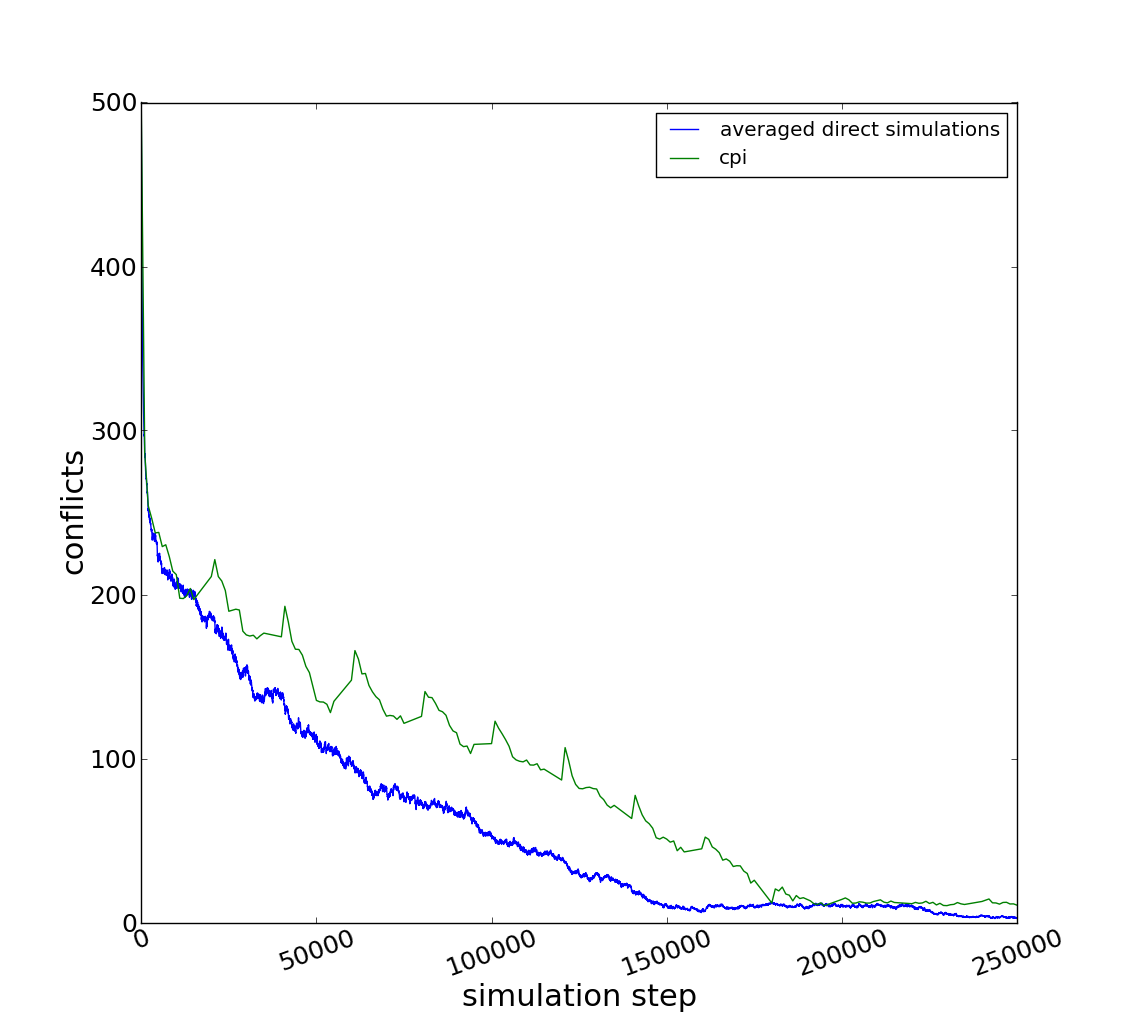
\includegraphics[height=65mm]{vmCPIFast1}
    \label{fig:vmFast1}
  }
  \hspace{3mm}
  \subfloat[Evolved $15,000$ steps, projected $10,000$.]{
    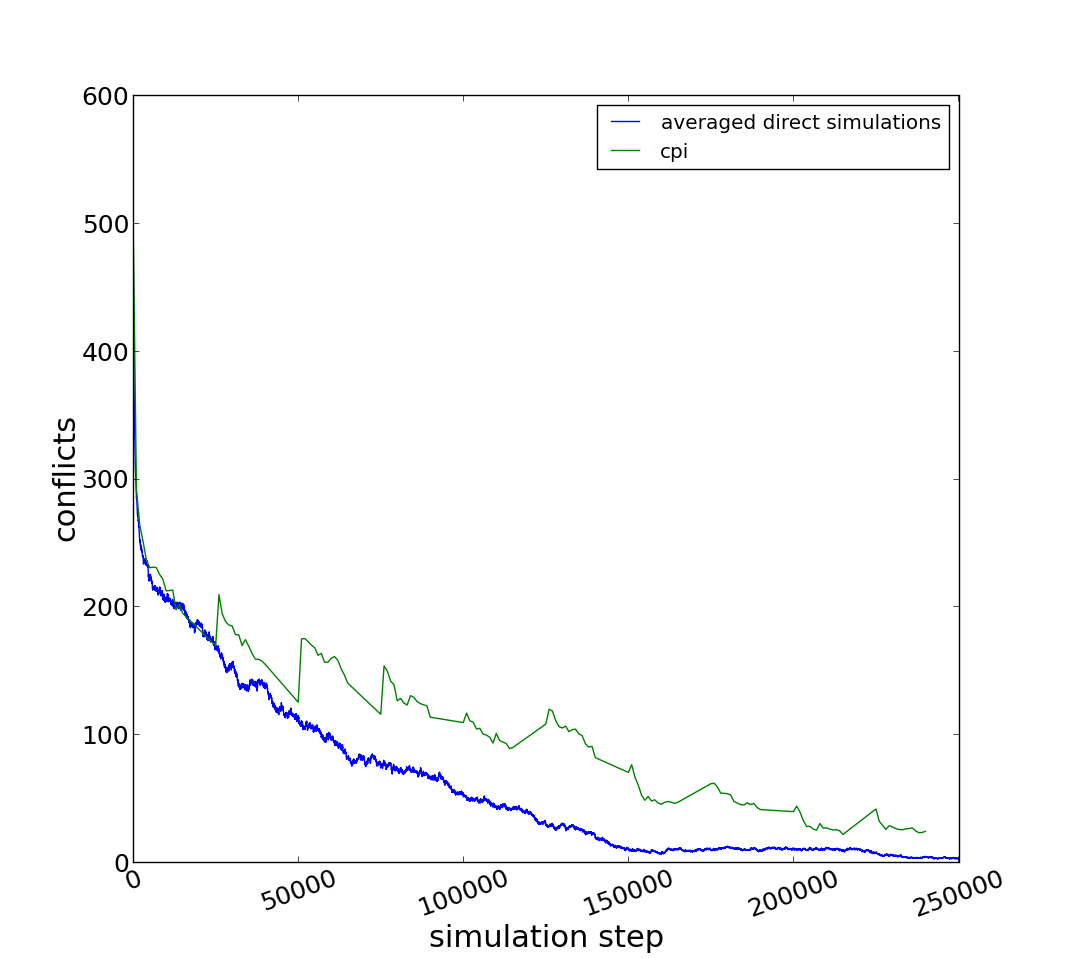
\includegraphics[height=65mm]{vmCPIFast2}
    \label{fig:vmFast2}
  }
  \caption{Second CPI method in which finished runs in the ensemble contribute their data to the projection step, but are no longer evolved in time. As this amounts to adding zero conflict runs to the ensemble, convergence is faster.}
  \label{fig:vmFast}
\end{figure}

\begin{figure}
  \centering
  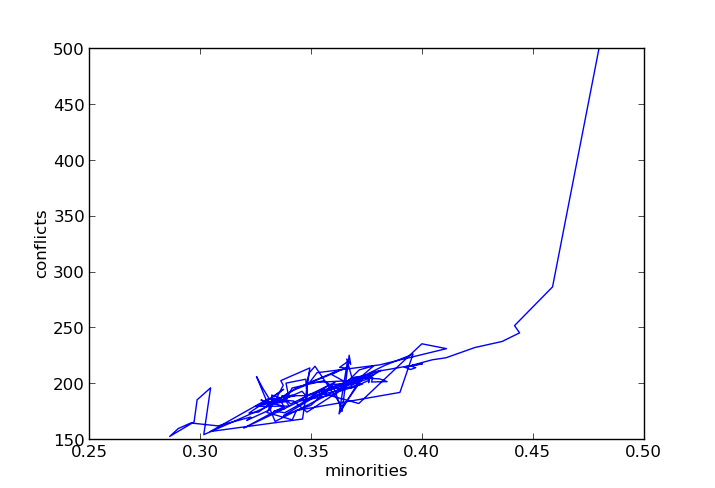
\includegraphics[height=65mm]{vmCPIPP}
  \caption{Phase portrait calculated with CPI, evolved $15,000$ steps, projected $10,000$.}
  \label{fig:vmPP}
\end{figure}

\section*{Edge reconnecting model}

\begin{figure}
  \centering
  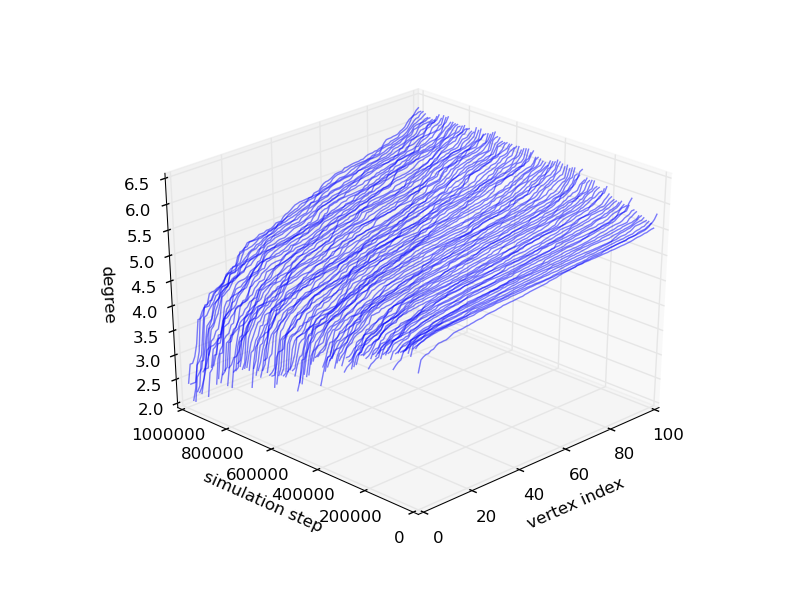
\includegraphics[height=65mm]{erQuadraticTimescale}
  \caption{Attempt to visualize the fast, $n^{2}$, timescale, on which the degree distribution is expected to remain constant.}
  \label{fig:erFast}
\end{figure}

\begin{figure}
  \centering
  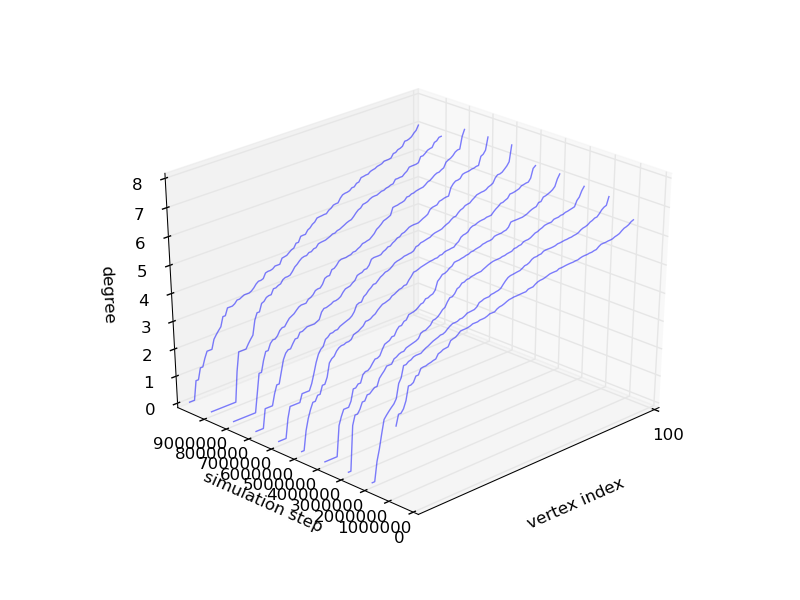
\includegraphics[height=65mm]{erCubicTimescale}
  \caption{Attempt to visualize the slower, $n^{3}$, timescale, on which the degree distribution should evolves to a steady state.}
  \label{fig:erSlow}
\end{figure}

\begin{figure}
  \centering
  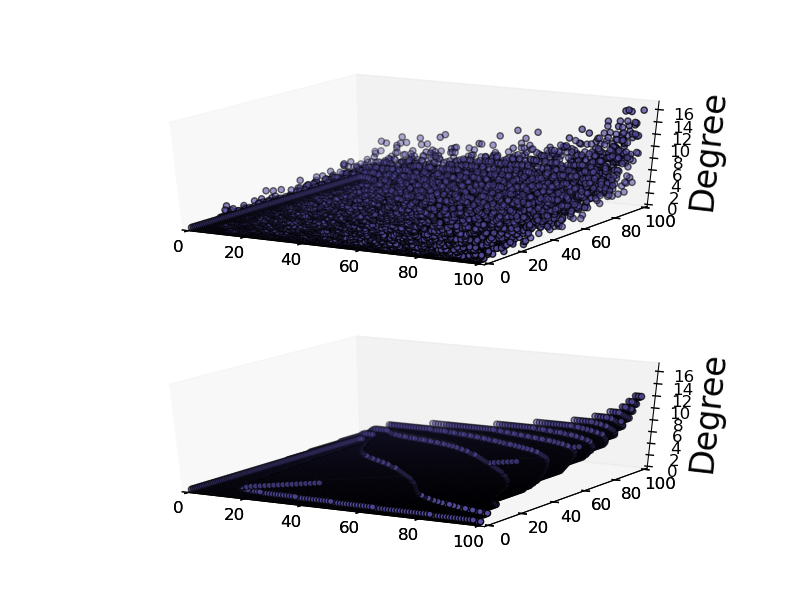
\includegraphics[height=65mm]{erRecon}
  \caption{Reconstruction of adjacency matrix using the leading eigenvector and eigenvalue.}
  \label{fig:erRecon}
\end{figure}

\begin{figure}
  \centering
  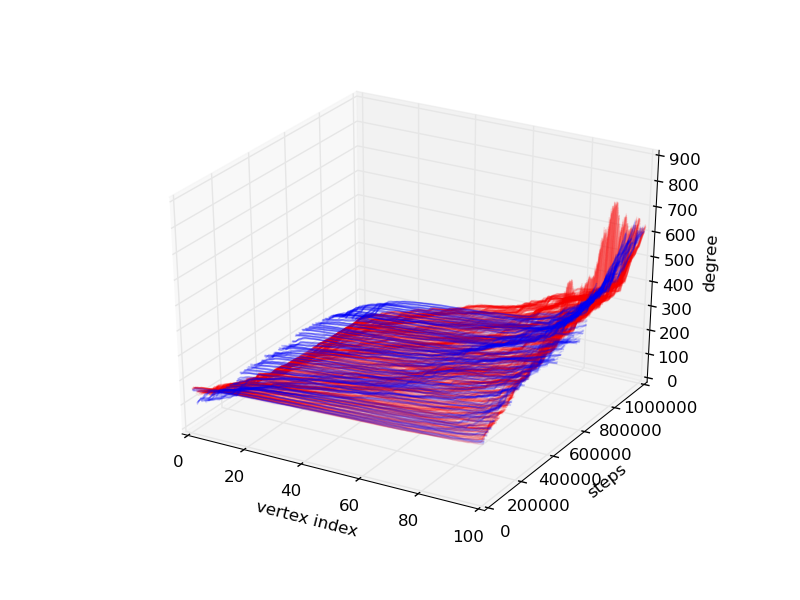
\includegraphics[height=65mm]{erCPI}
  \caption{Evolution of degree distribution during CPI (blue) and direct simulation (red).}
  \label{fig:erRecon}
\end{figure}

\begin{figure}
  \centering
  \subfloat[1st Coeff.]{
    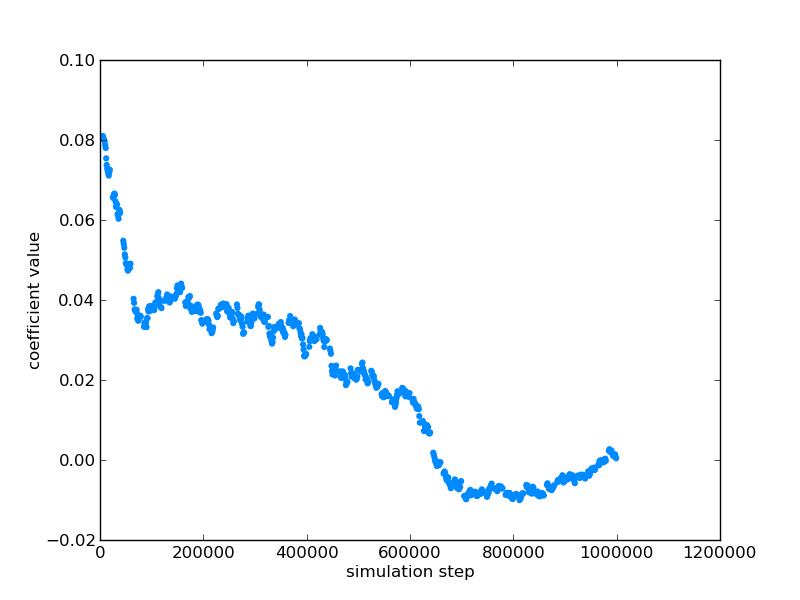
\includegraphics[height=65mm]{coeff0}
    \label{fig:er1Coef}
  }
  \subfloat[2nd Coeff.]{
    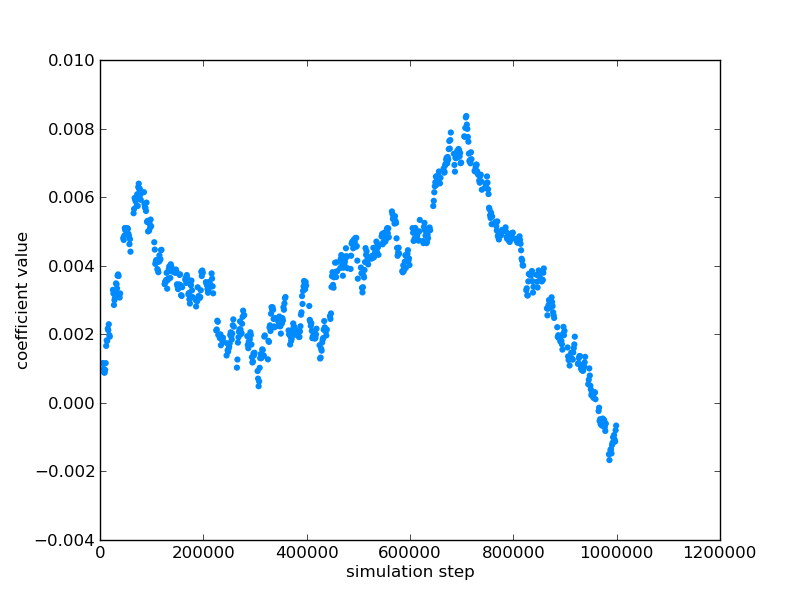
\includegraphics[height=65mm]{coeff1}
    \label{fig:er2Coef}
  }
  \hspace{3mm}
  \subfloat[3rd Coeff.]{
    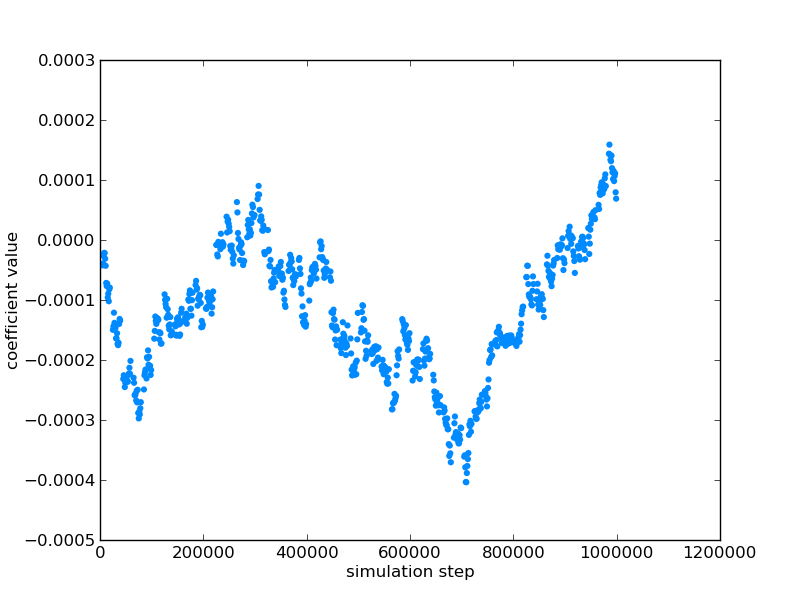
\includegraphics[height=65mm]{coeff2}
    \label{fig:er3Coef}
  }
  \subfloat[4th Coeff.]{
    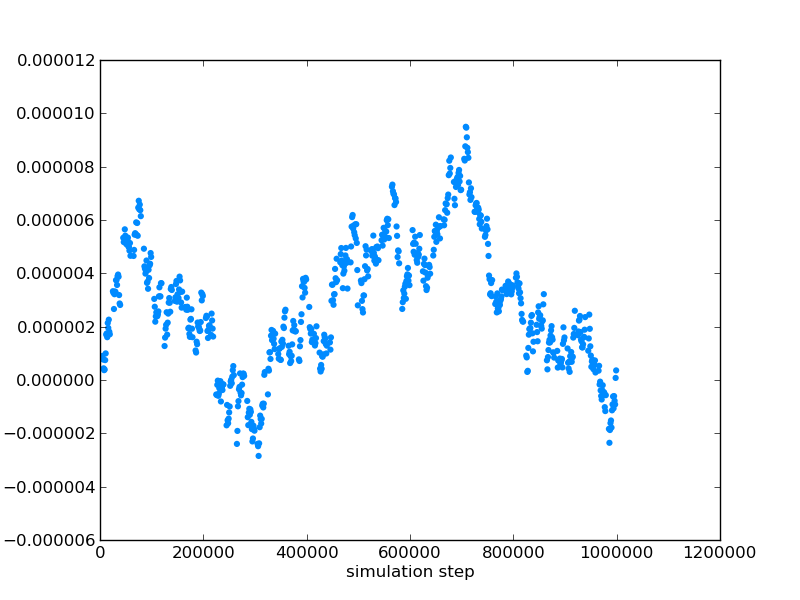
\includegraphics[height=65mm]{coeff3}
    \label{fig:er4Coef}
  }
  \hspace{3mm}
  \subfloat[5th Coeff.]{
    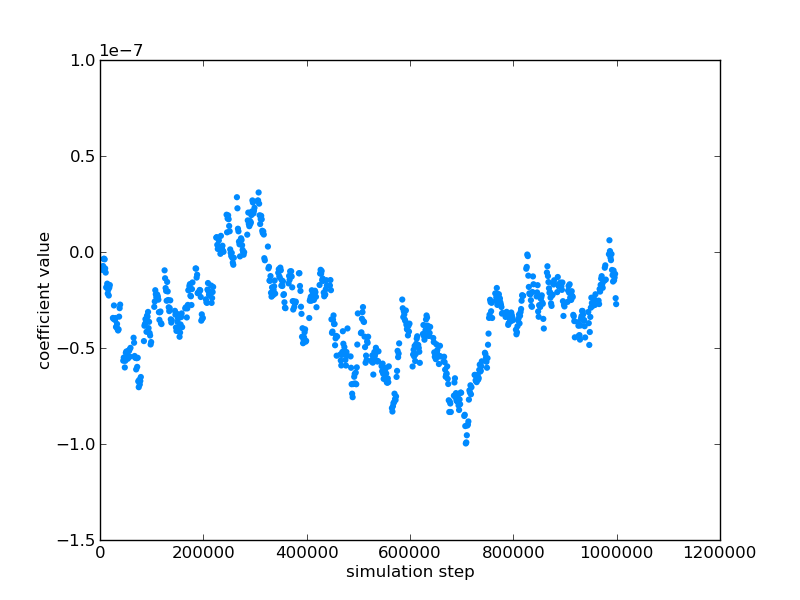
\includegraphics[height=65mm]{coeff4}
    \label{fig:er5Coef}
  }
  \caption{Evolution of coefficients used to fit first eigenvector of adjacency matrix, which were used as coarse variables.}
  \label{fig:erCoeff}
\end{figure}

%% \begin{figure}
%%   \centering
%%   \subfloat[Only includes runs that have reached consensus]{
%%     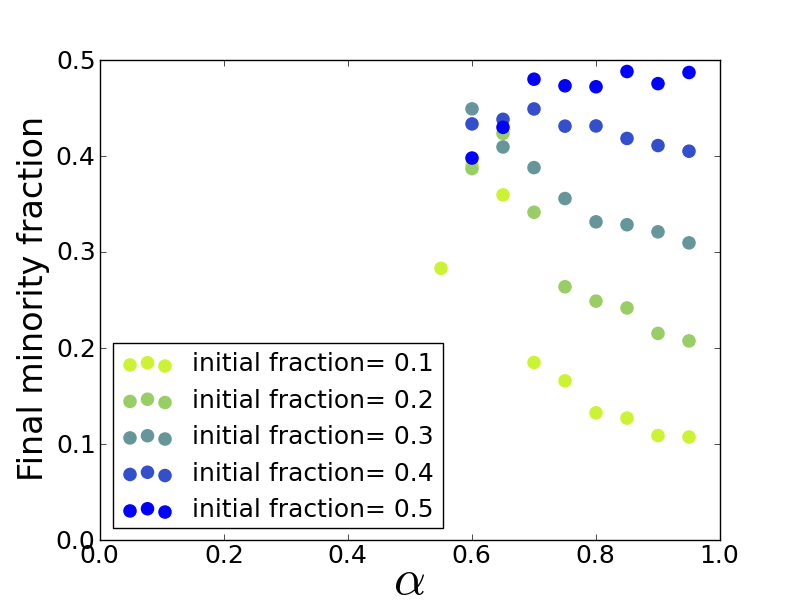
\includegraphics[width=72mm]{bifData_same_1000_4}
%%     \label{fig:rwSameA}
%%   }
%%   \hspace{3mm}
%%   \subfloat[Includes all runs, even if conflicts exist at the simulation's end] {
%%     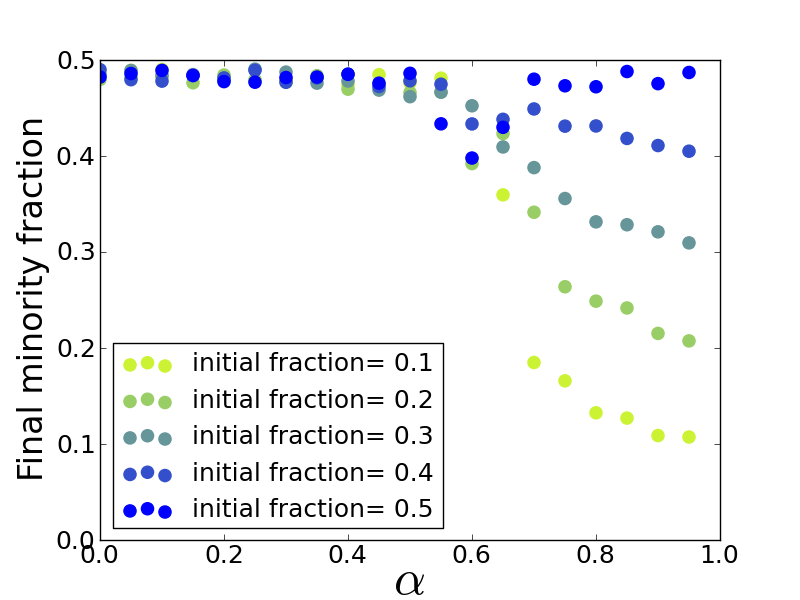
\includegraphics[width=72mm]{bifData_noConvergence_same_1000_4}
%%     \label{fig:rwSameB}
%%   }
%%   \caption{Final minority fraction as a function of $\alpha$ and initial minority fraction (rewire-to-same), results from our data.}
%%   \label{fig:myRWtoSameBD}
%% \end{figure}

\end{document}
